\documentclass[11pt]{article}
\usepackage[margin=1in]{geometry}
\usepackage[T1]{fontenc}
\usepackage{lmodern}
\usepackage{microtype}
\usepackage{hyperref}
\usepackage{parskip}
\usepackage{graphicx}
\graphicspath{{figures/}}

\title{PermitKey: A harmonized national work-type classification of 150 million U.S. building permit records}
\author{Candy Martinez$^{\ast 1}$ \and Sean Hardesty Lewis$^{\dagger 1}$ \and Yichun Fan$^{\ddagger 2}$ \and Siqi Zheng$^{\S 1}$}
\date{}

\begin{document}
\maketitle
\begin{center}
$^{1}$Sustainable Urbanization Lab and Center for Real Estate, Massachusetts Institute of Technology, Cambridge, MA, USA\\
$^{2}$Nicholas School of the Environment, Duke University, Durham, NC, USA
\end{center}

\begin{abstract}
Building permits are among the most complete records of physical change to the U.S. built environment, but they cannot be compared across jurisdictions. Local authorities classify work for administrative purposes, using vocabularies that differ in granularity and share few common definitions. The national Building Permits Survey counts newly authorized housing units, leaving most work on the existing stock unmeasured.

PermitKey contributes a general procedure and a national reference implementation. The procedure treats jurisdiction-supplied labels as weak supervision, trains a multi-label classifier over permit descriptions against an analyst-specified taxonomy, and validates the result against source labels and blind human review. The reference implementation retains 150,044,555 source-record occurrences from 85 contributions and assigns candidate labels under a documented 25-category work-type taxonomy. Derived products are designed for permitting-jurisdiction $\times$ year $\times$ work type and, where property locations are reliable, 0.1$^{\circ}$ grid $\times$ year $\times$ work type analysis. The release includes definitions, provenance, validation tables, and classification code while protecting raw permit-level records through aggregation and disclosure review.
\end{abstract}

\section{Background and summary}
Most of the buildings that will stand in the United States in 2050 have already been built. Whether the country decarbonizes its buildings, adapts them to a hotter and more hazardous climate, and houses a population with evolving ways of living and working therefore depends on what is done to the existing stock: kitchens remodeled, roofs replaced, accessory dwelling units added, electrical panels upgraded, heat pumps and rooftop solar installed, and structures hardened against wind, fire, and flood. The national statistical system sees little of this activity. The Census Bureau's Building Permits Survey collects from local permit offices primarily the count of newly authorized housing units.

The local records themselves are richer. Jurisdictions issue permits for new construction, alterations, additions, demolitions, roof replacements, electrical and mechanical work, and equipment installation. Public records are dated, tied to a property or jurisdiction, and often accompanied by free-text descriptions. Taken together, they provide a near-national view of physical change at the moment work is authorized.

The obstacle is comparability. Permit authorities classify work for administrative and fee-setting purposes, so source vocabularies differ by orders of magnitude in granularity. A national measure cannot be assembled by simply joining local labels. PermitKey addresses this problem by separating source preservation from analytic harmonization: native labels and provenance remain traceable, while a shared taxonomy supplies a common measurement frame.

\section{Data and method}
The current logical set contains 150,044,555 collected source-record occurrences across 85 contributions. Records are retained as published; the pipeline does not assume that a permit number is a globally unique identifier. Application, issue or approval, and source dates are preserved separately. Geographic fields are retained with their source provenance, and grid products are restricted to records that pass location-quality checks.

\begin{figure}[htbp]
  \centering
  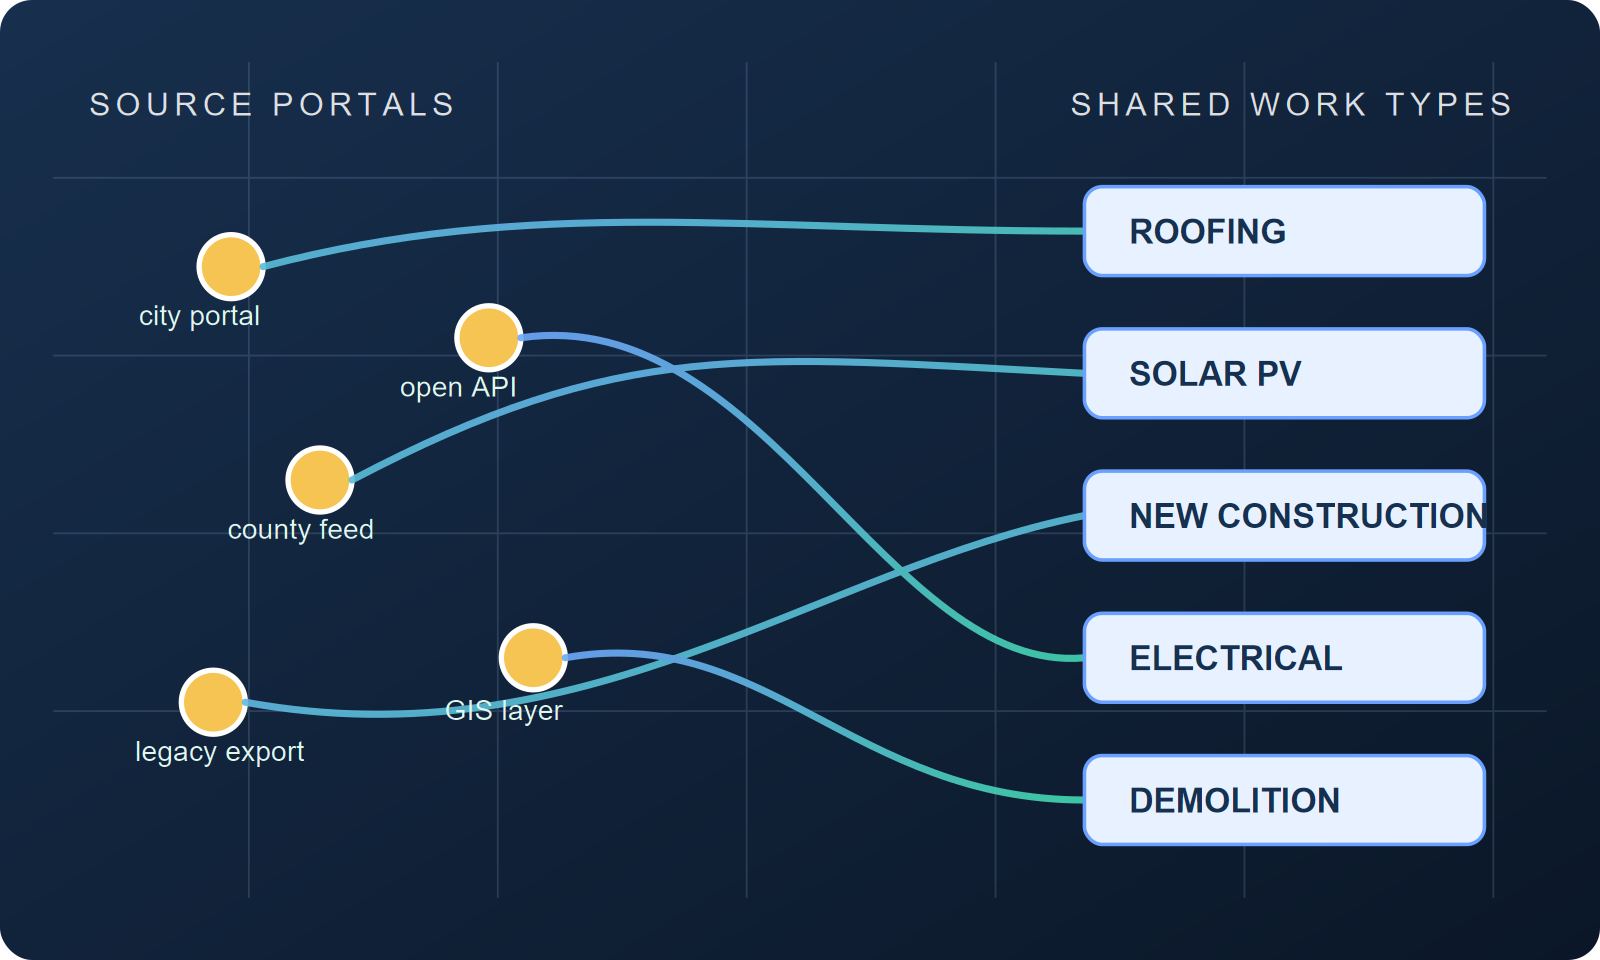
\includegraphics[width=\linewidth]{fig1-permitkey-overview.png}
  \caption{PermitKey overview. Heterogeneous local permitting portals are connected to a shared multi-label work-type vocabulary while source provenance and missingness remain traceable.}
  \label{fig:permitkey-overview}
\end{figure}

Source labels provide abundant but noisy supervision. We normalize descriptions and structured fields, train one independent classifier per work type, and permit multiple labels on a record. Multi-labeling is substantive: a single permit can authorize several related jobs, such as electrical work performed as part of a solar installation. The current Natural25 taxonomy spans construction, alteration, demolition, building systems, exterior work, sitework, and energy technologies.

Validation combines comparisons with municipal labels and adjudicated human review. The current audit contains 3,080 completed human judgments, with reviewer agreement reported separately from model performance. A historical held-out-city evaluation of the classification family reports micro-F1 of 0.874; final release estimates will be recomputed after the production label run and documented with class-specific uncertainty.

\begin{figure}[htbp]
  \centering
  \includegraphics[width=\linewidth]{fig1-national-distribution.webp}
  \caption{National distribution of building-permit records. Records with valid U.S. coordinates are aggregated to grid cells and displayed on a logarithmic color scale. Alaska, Hawaii, and Puerto Rico are shown as insets. The map depicts record density in the assembled corpus and does not imply complete permit coverage within populated cells.}
  \label{fig:national-distribution}
\end{figure}

\begin{figure}[htbp]
  \centering
  \includegraphics[width=\linewidth]{fig2-classification-workflow.webp}
  \caption{Permit work-type classification and development-validation workflow. Permit descriptions and record fields are transformed into multi-label work-type assignments, then evaluated with municipal weak labels, held-out-city rotation, and an external solar comparison. Displayed metrics are development estimates; final release metrics will be pinned to the frozen label run.}
  \label{fig:classification-workflow}
\end{figure}

\begin{figure}[htbp]
  \centering
  \includegraphics[width=\linewidth]{fig3-temporal-class-patterns.webp}
  \caption{Temporal patterns in selected permit classes. Lines show first-observed class-positive properties across stable reporting jurisdictions and directly geocoded cells, indexed to each series' 2012--2024 maximum. The panels illustrate how harmonized work types can expose technology adoption over time.}
  \label{fig:temporal-patterns}
\end{figure}

\begin{figure}[htbp]
  \centering
  \includegraphics[width=\linewidth]{fig4-spatial-technology-adoption.webp}
  \caption{Cumulative spatial distribution of permit-documented residential technologies through 2024. Solar PV, EV charging, air-source heat pumps, and home batteries are shown on a 0.25-degree grid with class-specific logarithmic scales. The EV panel is an observed lower bound.}
  \label{fig:technology-adoption}
\end{figure}

\section{Release design and reuse}
PermitKey is released as derived aggregate data rather than raw permit-level records. The primary table is indexed by permitting jurisdiction, year, and work type. A companion 0.1$^{\circ}$ grid table is provided only where property locations are sufficiently reliable; records located only to a jurisdiction remain in the jurisdiction-level product. Category counts may overlap because records can carry multiple work types. The release package includes a data dictionary, taxonomy definitions and examples, source contribution registry, provenance fields, validation tables, and the classification pipeline so that researchers can apply the procedure to new jurisdictions or alternative taxonomies.

These products support research on housing supply, retrofit and electrification, climate adaptation, construction cycles, neighborhood change, and the evaluation of policies such as building-performance standards and clean-energy incentives. They also provide a common starting point for city planning and urban-environment applications that currently require bespoke, single-jurisdiction cleaning.

\section{Limitations}
Coverage and field quality vary across jurisdictions and years. Source records are occurrences rather than deduplicated unique permits, and multi-label counts are not additive. Weak supervision inherits errors and omissions from local labels; human-review estimates and source-rights checks therefore remain part of the release protocol. Aggregate geography and disclosure rules are applied before publication, and the public release will state the eligible coverage and uncertainty for every table.

\section*{Data and code availability}
The public project page is available at \url{https://permitkey.github.io}. Aggregate tables, documentation, taxonomy definitions, validation results, and classification code will be published there as the release gates are completed. Raw permit-level records remain in the project working environment and are not part of the public release.

\end{document}
